\documentclass{article}

\usepackage{amsmath}
\usepackage{amssymb}
\usepackage{geometry}
\usepackage{hyperref}
\usepackage{parskip}
\usepackage{graphicx}
\usepackage{float}
\usepackage{tabularx}
\usepackage{mathtools}

\graphicspath{{../Images/}}

% \renewcommand\thesection{Problem \arabic{section}}
% \renewcommand\thesubsection{\arabic{subsection}}
\numberwithin{equation}{section}

\DeclarePairedDelimiter\ceil{\lceil}{\rceil}
\DeclarePairedDelimiter\floor{\lfloor}{\rfloor}

\DeclareMathOperator*{\trace}{trace}
\DeclareMathOperator*{\rank}{rank}
\newcommand{\AHA}[1]{#1\hermit #1}
\newcommand{\norm}[2][]{\Vert #2\Vert_{#1}}
\newcommand{\hermit}{^H}
\newcommand{\transpose}{^T}
\newcommand{\inverse}{^{-1}}
\newcommand{\ATA}[1]{#1\transpose #1}
\newcommand{\at}[2][]{#1|_{#2}}
\DeclareMathOperator{\EX}{\mathbb{E}}% expected value
\DeclareMathOperator*{\argmax}{arg\,max}
\DeclareMathOperator*{\argmin}{arg\,min}
\DeclareMathOperator*{\MSE}{MSE}

\title{Deep Learning - Assignment 3}
\author{Ali Abbasi}
\begin{document}
\maketitle

\section{}
\subsection{}
The result of this convolution is as follows (see theory.ipynb):
\begin{figure}[H]
\centering
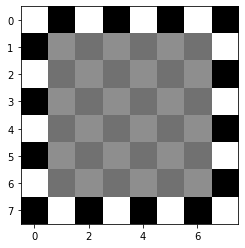
\includegraphics[width=0.3\textwidth]{theory-1.png}
\caption{Result of convolution.}
\end{figure}
where the edge pixels are preserved as mentioned.
\subsection{}
This filter act similar to a average pooling filter with \(kernel_size=(3, 3)\), where each pixel is replaced by the average of its 8 neighbors and itself.

\section{}
Dimension of input of the size \(H \times W \times C\) after a Conv\(k-N(S, P)\) layer is \(H' \times W' \times N\), where:

\begin{align}
H' &= \floor*{\frac{H - k + 2P}{S}} + 1 \\
W' &= \floor*{\frac{W - k + 2P}{S}} + 1
\end{align}

\begin{table}[H]
\centering
\begin{tabular}{|c|c|c|}
\hline 
Layer & Output Dimension & Parameters \\
\hline
Input & \(32 \times 32 \times 3\) & 0 \\
\hline
CONV3-10 & \(32 \times 32 \times 10\) & \(3 \times 3 \times 3 \times 10 + 10\) \\
\hline
ReLU & \(32 \times 32 \times 10\) & 0 \\
\hline
POOL-2 & \(16 \times 16 \times 10\) & 0 \\
\hline
CONV3-20(3,2) & \(6 \times 6 \times 20\) & \(3 \times 3 \times 10 \times 20 + 20\) \\
\hline
ReLU & \(6 \times 6 \times 20\) & 0 \\
\hline
POOL-2 & \(3 \times 3 \times 20\) & 0 \\
\hline
FLATTEN & \(180\) & 0 \\
\hline
FC-10 & \(10\) & \(180 \times 10 + 10\)\\
\hline
\end{tabular}
\end{table}

\section{}
\subsection{}
\(k_1, k_2, k_3\), \(b\), \(w_1, w_2\) and \(a\) are the parameters of the network.
\subsection{}
\begin{align}
\hat{y} &= w_1v_1 + w_2v_2 + b \\
L &= \frac{1}{2}(y - \hat{y})^2
\end{align}
\begin{align}
\frac{\partial L}{\partial \hat{y}} &= \hat{y} - y \\
\frac{\partial L}{\partial a} &= \frac{\partial L}{\partial \hat{y}} \frac{\partial \hat{y}}{\partial a} \\
&= \hat{y} - y\\
\frac{\partial L}{\partial w_1} &= \frac{\partial L}{\partial \hat{y}} \frac{\partial \hat{y}}{\partial w_1} \\
&= (\hat{y} - y)v_1\\
\frac{\partial L}{\partial w_2} &= \frac{\partial L}{\partial \hat{y}} \frac{\partial \hat{y}}{\partial w_2} \\
&= (\hat{y} - y)v_2
\end{align}

\subsection{}
\begin{align}
\frac{\partial L}{\partial v_1} &= \delta_1 \\
\frac{\partial L}{\partial v_2} &= \delta_2 \\
\frac{\partial L}{\partial z_1} &=
\begin{cases}
\delta_1 & \text{if } z_1 > 0 \text{ and } z_1 \ge z_2 \\
0 & \text{otherwise}
\end{cases}\\
\frac{\partial L}{\partial z_2} &=
\begin{cases}
\delta_1 & \text{if } z_2 > 0 \text{ and } z_2 > z_1 \text{ and } z_2 \le z_3 \\
\delta_2 & \text{if } z_2 > 0 \text{ and } z_2 \le z_1 \text{ and } z_2 > z_3 \\
\delta_1 + \delta_2 & \text{if } z_2 > 0 \text{ and } z_2 > z_1 \text{ and } z_2 > z_3 \\
0 & \text{otherwise}
\end{cases}\\
\frac{\partial L}{\partial z_3} &=
\begin{cases}
\delta_2 & \text{if } z_3 > 0 \text{ and } z_3 \ge z_2 \\
0 & \text{otherwise}
\end{cases}\\
\end{align}
(Assuming ties are broken in favor of \(z_1\) and \(z_3\)).

\subsection{}
\begin{align}
\frac{\partial L}{\partial k_1} &= \alpha_1 x_1 + \alpha_2 x_2 + \alpha_3 x_3 \\
\frac{\partial L}{\partial k_2} &= \alpha_1 x_2 + \alpha_2 x_3 + \alpha_3 x_4 \\
\frac{\partial L}{\partial k_3} &= \alpha_1 x_3 + \alpha_2 x_4 + \alpha_3 x_5\\
\frac{\partial L}{\partial b} &= \alpha_1 + \alpha_2 + \alpha_3
\end{align}

\subsection{}
\begin{align}
\frac{\partial L}{\partial k_j} &= \alpha_1 x_{j} + \alpha_2 x_{j+1} + \cdots + \alpha_{m} x_{n - d + j} \\
\frac{\partial L}{\partial b} &= \alpha_1 + \alpha_2 + \cdots + \alpha_{m}
\end{align}

\section{}
\subsection{}
Since the kernel acts similarly on width and height of the input, it is a square kernel.
\begin{align}
\frac{205 - k}{3} + 1 = 66 \\
\implies k = 205 - 65 \times 3 = 10
\end{align}
So it is a convolution with \(96\) kernels of size \(10 \times 10 \times 10\) (since the input's channel size is \(10\)) with stride \(3\).
\subsection{}
\begin{align}
96 \times 10 \times 10 \times 10 + 96 = 96,096
\end{align}
\subsection{}
For each output value, \(10 \times 10 \times 10\) multiplications are performed. So the number of multiplications is:
\begin{align}
66 \times 66 \times 96 \times 10 \times 10 \times 10 = 418,176,000
\end{align}


\end{document}